\chapter{The Sun}\label{csun}
% !TEX root = ./Almagest.tex

\section{Solar Ecliptic Longitude Model}
Our solar longitude model is sketched in Figure~\ref{lf3}. From a geocentric point of view, the Sun, $S$,  appears to execute
a (counterclockwise) Keplerian orbit of major radius $a$, and eccentricity $e$, about the
Earth, $G$. As has already been mentioned, the circle traced out by the Sun on the celestial sphere is
known as the  ecliptic circle. This circle is inclined at $23^\circ 26'$ to
the celestial equator, which is the projection of the Earth's equator onto
the celestial sphere.
 Suppose that the angle subtended at the Earth between the vernal equinox (that is, the point at which the ecliptic crosses the celestial equator from
south to north) and the
Sun's perigee (that is, the point of closest approach to the Earth)   is
 $\varpi$. This
angle is termed the {\em longitude of the perigee}, and
 is assumed
to vary  linearly with time: that is, 
\begin{equation}\label{ae79}
\varpi  = \varpi_0 + \varpi_1\,(t-t_0).
\end{equation}

\begin{figure}[h]
\centerline{\includegraphics[height=3in]{Fig5-1.eps}}
\caption{The apparent orbit of the Sun about the Earth.  Here, $S$, $G$, $\Pi$, $A$, $\varpi$, $T$,  $\lambda$, and $\Upsilon$
represent the Sun, the Earth, the perigee, the apogee, the longitude of the perigee, the true anomaly, the ecliptic longitude, and
The vernal equinox, respectively. the view is from northern ecliptic pole. The Sun orbits counterclockwise.}\label{lf3}
\end{figure}

 The Sun's {\em ecliptic
longitude}\/ is defined as the angle subtended at the Earth between the vernal equinox and the Sun.
Hence, from Figure~\ref{lf3},
\begin{equation}
\lambda = \varpi + T,
\end{equation}
where $T$ is the true anomaly. (See Chapter~\ref{ckep}.) By analogy, the  {\em mean longitude}\/ is written
\begin{equation}
\bar{\lambda} = \varpi + M,
\end{equation}
where $M$ is the  mean anomaly. (See Chapter~\ref{ckep}.) It follows from Equation~(\ref{je23}) that
\begin{equation}\label{ae82}
\lambda = \bar{\lambda}  + q,
\end{equation}
where
\begin{equation}
q = 2\,e\,\sin M + (5/4)\,e^2\,\sin\,2M,
\end{equation}
 is called  the {\em equation of  center}. Note that $\lambda$, $\bar{\lambda}$, $T$, and $M$ are usually written as angles in the range
 $0^\circ$ to $360^\circ$, whereas $q$ is generally written as an
 angle in the range $-180^\circ$ to $+180^\circ$. 

The mean longitude increases
uniformly with time (because both $\varpi$ and $M$ increase uniformly with time) as
\begin{equation}\label{ae84}
\bar{\lambda} =  \bar{\lambda}_0+ n\,(t -t_0),
\end{equation}
where $\bar{\lambda}_0$ is termed the
{\em mean longitude at epoch}, 
$n$ the {\em rate of motion in mean longitude}, and $t_0$ the {\em epoch}. 
We can also write
\begin{equation}\label{ae85}
M = M_0 + \tilde{n}\,(t-t_0),
\end{equation}
where
\begin{equation}
M_0 = \bar{\lambda}_0 - \varpi_0
\end{equation}
is called the {\em mean anomaly at epoch}, and 
\begin{equation}\label{ae87}
\tilde{n} = n - \varpi_1
\end{equation}
 the {\em rate of motion in mean anomaly}. 
 
 Our procedure for determining the ecliptic longitude of the Sun is as follows.
 The requisite orbital elements (that is, $e$, $n$, $\tilde{n}$, $\bar{\lambda}_0$, and $M_0$) for the J2000 epoch (that is, 12:00 UT on January 1, 2000 AD/, which corresponds to $t_0= 2\,451\,545.0$ JD) are listed
in Table~\ref{lt4}. These elements are calculated
on the assumption that the vernal equinox  precesses at the uniform
rate of $-3.8246\times 10^{-5}\,\,^\circ/{\rm day}$. 
The ecliptic longitude of the Sun is specified by the
following formulae:
\begin{align}
\bar{\lambda} &=  \bar{\lambda}_0+ n\,(t-t_0),\\[0.5ex]
M &= M_0 + \tilde{n}\,(t-t_0),\\[0.5ex]
q &= 2\,e\,\sin M + (5/4)\,e^2\,\sin\,2M,\label{le2.8}\\[0.5ex]
\lambda &= \bar{\lambda}  + q.
\end{align}
 These formulae are capable of matching NASA ephemeris data\,\footnote{See {\tt http://ssd.jpl.nasa.gov/}}
during the years 1995--2006 AD with a mean error of $0.2'$ and a maximum error of $0.7'$. 

The ecliptic longitude of the Sun can be calculated with the aid of Tables~\ref{lt5} and \ref{lt6}.
 Table~\ref{lt5} allows the mean longitude, $\bar{\lambda}$, and mean anomaly,
 $M$, of the
Sun to be determined as  functions of time. Table~\ref{lt6} specifies the equation of center, $q$, as a
function of the mean anomaly. 

 Note that Table~\ref{lt5} contains essentially the same information as that contained in the ``Table of the Sun's mean motion" (Κανόνιον τῆς ὁμαλῆς τοῦ ἡλίου κινήσεως) that appears in
 Section~2 of Book~III of the Almagest. Likewise, Table~\ref{lt6} contains essentially the same information as that contained in the ``Table of the solar anomaly'' (Κανόνιον τῆς  ἡλιακῆς ἀνωμαλίας)
 that appears in Section~6 of Book~III of the Almagest.
 
\section{Determination of Solar Ecliptic Longitude}\label{ssun}
The procedure for using Tables~\ref{lt5} and \ref{lt6} to determine solar longitude  is as follows:
\begin{enumerate}

\item Determine the fractional Julian day number, $t$, corresponding to the date and time
at which the Sun's ecliptic longitude is to be calculated with the aid of Tables~\ref{kt1}--\ref{kt3}. Form $\Delta t = t-t_0$, where $t_0=2\,451\,545.0$ is the epoch. 

\item Enter Table~\ref{lt5} with the digit for each power of 10
in ${\Delta} t$ and take out the corresponding values of $\Delta\bar{\lambda}$ and $\Delta M$. If $\Delta t$ is negative then the corresponding
values are also negative.
The value of the mean longitude, $\bar{\lambda}$, is the
sum of all the $\Delta\bar{\lambda}$ values plus the value of $\bar{\lambda}$ at the epoch. Likewise, the value of the mean anomaly, $M$, is
the sum of all the $\Delta M$ values plus the value of $M$ at the epoch. 
Add as many multiples of $360^\circ$ to $\bar{\lambda}$ and $M$
as is required to make them both fall in the range $0^\circ$ to $360^\circ$. Round $M$ to the nearest degree. 

\item Enter Table~\ref{lt6} with the value of $M$ and take out the
corresponding value of the equation of center, $q$, and the radial anomaly, $\zeta$. (The latter step is only necessary if the ecliptic longitude of the Sun is
to be used to determine that of a planet.) It is necessary to interpolate if $M$ is odd.

\item The ecliptic longitude, $\lambda$, is the sum of the mean longitude, $\bar{\lambda}$, and the equation of center, $q$. If necessary, convert $\lambda$ into an angle in the range $0^\circ$ to $360^\circ$. 
The decimal fraction can be converted into arc minutes
using Table~\ref{lt6a}. Round to the nearest arc minute. 
\end{enumerate}
Two examples of the use of this procedure are given in the next section.

\section{Example Solar Longitude Calculations}
\noindent {\em Example 1}: May 5, 2005 AD, 00:00 UT:\\
~\\
According to Tables~\ref{kt1}--\ref{kt3}, $t = 2\,453\,495.5$ JD. Hence,
$t-t_0 = 2\,453\,495.5-2\,451\,545.0=1\,950.5$ JD. Making use of
Table~\ref{lt5}, we find:\\
\begin{tabular}{rrr}
&&\\
$t$(JD) & $ \bar{\lambda}(^\circ)$ & $M(^\circ)$\\[-2ex]
&&\\
$+1\,000$ & $265.647$ & $265.600$\\
$+900$ & $167.083$ & $167.040$\\
$+50$ & $49.282$ & $49.280$\\
$+.5$ & $0.493$ & $0.493$\\
Epoch & $280.458$ & $357.588$\\\cline{2-3}
&$762.963$ & $840.001$\\\cline{2-3}
Modulus & $42.963$ & $120.001$\\ 
&&\\
\end{tabular}\\
Rounding the mean anomaly to the nearest degree, we obtain $M\simeq 120^\circ$.
It follows from  Table~\ref{lt6} that
$$
q(120^\circ)= 1.641^\circ,
$$ 
so
$$
\lambda =\bar{\lambda} + q =42.961+ 1.641=44.602\simeq 44^\circ36'.
$$
Here, we have converted the decimal fraction into arc
minutes using Table~\ref{lt6a}, and 
then rounded the final result to the nearest arc minute.

 Following
the practice of the Ancient Greeks (and modern-day astrologers), we shall express ecliptic longitudes
in terms of the  signs of the zodiac, which  are listed in Section~\ref{szod}. The ecliptic longitude $44^\circ36'$ is conventionally written 14TA36;  that is, 
$14^\circ36'$ into the sign of Taurus. Thus, we conclude that the position of
the Sun 
at 00:00 UT on May 5, 2005 AD was 14TA36.

~\\
\noindent {\em Example 2}: December 25, 1800 AD, 00:00 UT:\\
~\\
According to Tables~\ref{kt1}--\ref{kt3}, $t = 2\,378\,854.5$ JD. Hence,
$ t-t_0 = 2\,378\,854.5-2\,451\,545.0=-72\,690.5$ JD. Making use of
Table~\ref{lt5}, we find:\\
\begin{tabular}{rrr}
&&\\
$t$(JD) & $\bar{\lambda}(^\circ)$ & $ M(^\circ)$\\[-2ex]
&&\\
$-70\,000 $& $-235.315$ & $-232.017$\\
$-2\,000$ & $-171.295$ & $-171.200$\\
$-600$ & $-231.388$ & $-231.360$\\
$-90$ & $-88.708$ & $-88.704$\\
$-.5$ & $-0.493$ & $-0.493$\\
Epoch & $280.458$ & $357.588$\\\cline{2-3}
&$-446.741$ & $-366.186$\\\cline{2-3}
Modulus & $273.259$ & $353.814$\\
&&\\
\end{tabular}\\
We conclude that  $M\simeq 354^\circ$. 
 From Table~\ref{lt6}, 
$$
q(354^\circ)= -0.204^\circ,
$$  
so
$$
\lambda =\bar{\lambda} + q = 273.259 - 0.204=273.055\simeq 273^\circ03'.
$$
 Thus, the position of the Sun at 00:00 UT on December 25, 1800 AD was 3CP03. 
 
\section{Determination of Equinox and Solstice Dates}
We can also use Tables~\ref{lt5} and \ref{lt6} to calculate the dates of the equinoxes and solstices,
and, hence, the lengths of the seasons, in a given year. The {\em vernal equinox}\/ (that is, the point on the Sun's apparent orbit at which it passes through the celestial equator
from south to north)
corresponds to $\lambda=0^\circ$, the {\em summer solstice}\/ (that is, the
point at which the Sun is farthest north of the celestial equator) to $\lambda=90^\circ$, the {\em autumnal equinox}\/ (that is, the point at which the
Sun passes through the celestial equator from north to south) to $\lambda = 180^\circ$, and the
{\em winter solstice}\/ (that is, the point at which the Sun is farthest south of the celestial equator) to $\lambda = 270^\circ$. See Figure~\ref{lf6a}. Furthermore, {\em spring}\/ is defined as the period between the spring
equinox and the summer solstice, {\em summer}\/ as the period between the summer solstice and
the autumnal equinox, {\em autumn}\/ as the period between the autumnal equinox and the
winter solstice, and {\em winter}\/ as the period between the winter solstice and the following
vernal equinox. Consider the year 2000 AD.
For the case of the vernal equinox, we can
 first estimate the
 time at which this event takes place by approximating the solar
 longitude as the  mean
solar longitude; that is, 
$$
\lambda\simeq \bar{\lambda} = \bar{\lambda}_0 + n\,(t-t_0)
= 280.458 +  0.98564735\,(t-t_0),
$$
 We obtain 
$$
t \simeq t_0+(360-280.458)/0.98564735 \simeq t_0+81\,{\rm JD}.
$$ 
Calculating the true solar longitude at this time, using Tables~\ref{lt5} and \ref{lt6}, we get  
$\lambda = 2.177^\circ.$ Now, the actual vernal equinox occurs
when $\lambda=0^\circ$.
Thus, a much better estimate for the date of the vernal equinox
is
$$
t = t_0 + 81 -2.177/0.98564735 \simeq t_0 + 78.8\,{\rm JD},
$$
 which
corresponds to 7:00 UT on March 20. Similar calculations show that the summer solstice takes place at 
$$
t = t_0+ 171.6\, {\rm JD},
$$
corresponding to 2:00 UT on June 21, that the autumnal equinox
takes place at 
$$
t = t_0+265.2\,{\rm JD},
$$
corresponding to 17:00 UT
on September 22, and that the winter solstice takes place at
$$
t =t_0+355.1\, {\rm JD},
$$
corresponding to 14:00 UT on December 21. 
Thus, the length of spring is $92.8$ days,
the length of summer $93.6$ days,
and the length of autumn  $89.9$ days.
Finally, the length of winter is the length
of the tropical year (that is, the time period between successive vernal equinoxes), which is $360/0.98564735 = 325.24$ days, minus the sum of the lengths of the
other three seasons. This gives $88.9$ days. 

\begin{figure}[t]
\centerline{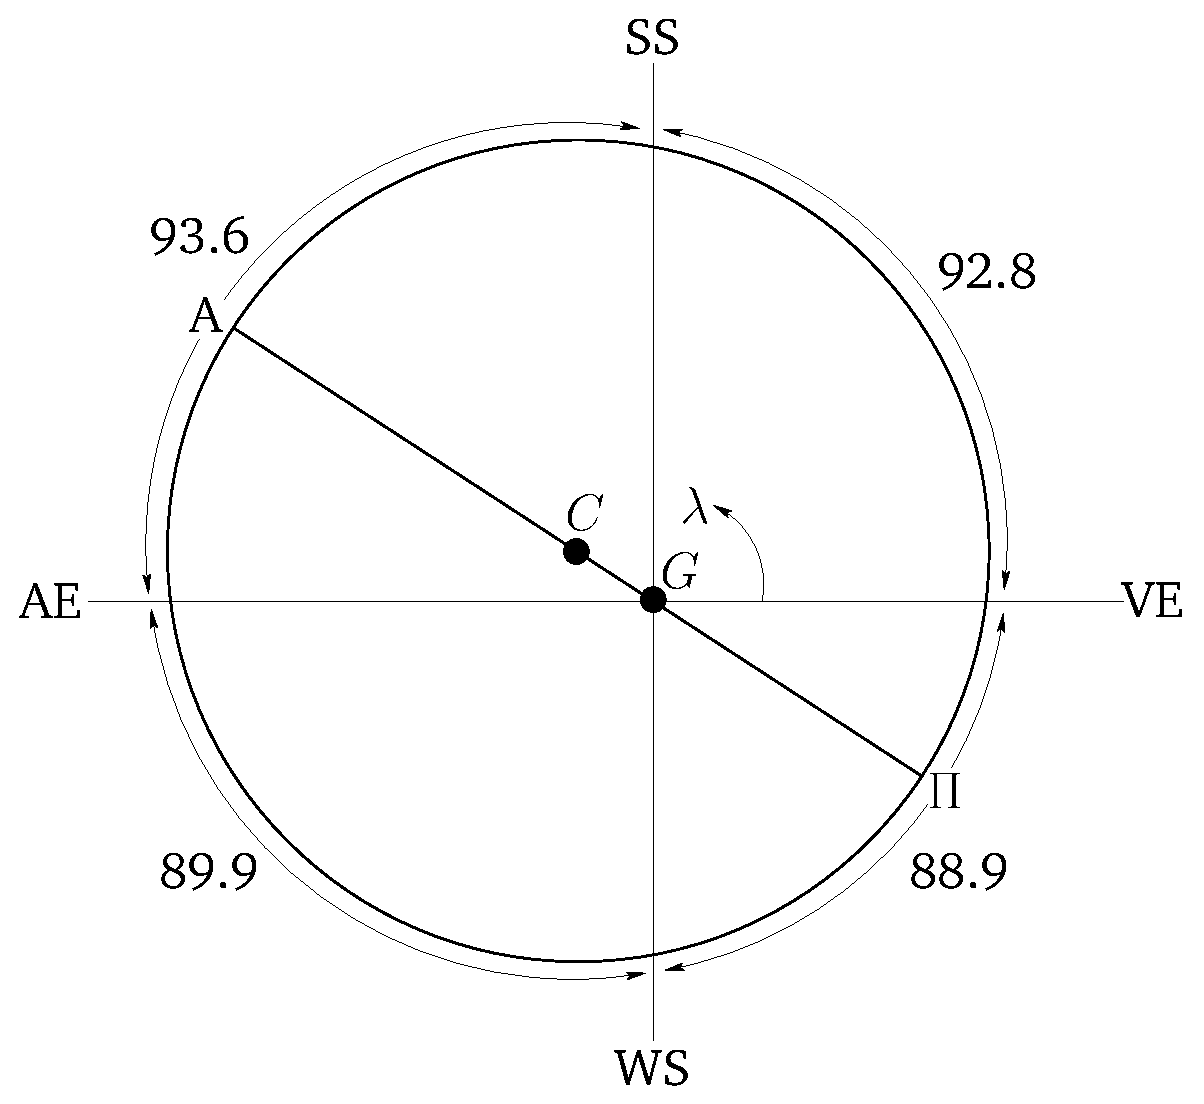
\includegraphics[height=3.5in]{Fig5-2.eps}}
\caption{The Sun's apparent orbit around the Earth, $G$, showing the vernal equinox (VE), summer
solstice (SS), autumnal equinox (AE), and winter solstice (WS). Here, $\lambda$, $\Pi$, $A$, and $C$
are the ecliptic longitude, the perigee, the apogee, and the geometric center of the orbit, respectively. The lengths
of the seasons (in days) are  indicated. }\label{lf6a}   
\end{figure}

Figure~\ref{lf6a} illustrates the relationship between the equinox and solstice points, and the
lengths of the seasons. The Earth is displaced from the geometric center of the Sun's apparent orbit in the direction of
the solar perigee, which presently lies between the winter solstice and the vernal equinox. This displacement (which is
greatly exaggerated in the figure) has
two effects. Firstly, it causes the arc of the Sun's apparent orbit between the summer solstice and autumnal equinox
to be longer than that between the winter solstice and the vernal equinox. Secondly, it causes the
Sun to appear to move faster in winter than in summer, in accordance with Kepler's second law, because the Sun is closer to the Earth in the
former season. Both of these effects tend to lengthen summer, and
shorten winter. Hence, summer is presently the longest season, and winter the shortest.

In Section~4 of Book~III of the Almagest, Ptolemy effectively performs the calculation described in this section in reverse, in order to determine the eccentricity of the Sun's
apparent orbit about the Earth, as well as the location of the solar perigee,  from the observed differences in the lengths of the seasons. However, Ptolemy's figures for the lengths of spring, summer, autumn, and winter,
which he inherited from Hipparchus,  were
94.5, 92.5, 88.125, and 90.125 days, respectively. The lengths of the seasons have changed since the time of Hipparchus because the solar perigee has
rotated by about $38^\circ$ (in the direction of the Sun's apparent motion) over the last 2\,200 years. 

\section{Equation of Time}
At any particular observation site on the Earth's surface, {\em local noon}\/
is defined as the instant in time when the Sun culminates at the
meridian. However, as a consequence of the inclination of the
ecliptic to the celestial equator, as well as the uneven motion of the
Sun around the ecliptic, the time interval  between successive local noons, which
is known as a {\em solar day}, 
is not constant, but varies throughout the year. Hence, if we were to
define a second as $1/86\,400$ of a solar day then the length of a second
would also vary throughout the year, which is clearly undesirable. In
order to avoid this problem, astronomers have invented a fictitious
body called the {\em mean Sun}. The mean Sun travels around the
celestial equator (from west to east) at a constant
rate that is such that it completes one orbit every tropical year. Moreover,
the mean Sun and the true Sun coincide at the spring equinox. {\em Local mean noon}\/ at a particular observation
site is defined as the instance in time when the mean Sun culminates at
the meridian. Because the orbit of the mean Sun is not inclined to the
celestial equator, and the mean Sun travels  around the celestial equator at a uniform rate, the time
interval between successive mean noons, which is known as a
{\em mean solar day}, takes the constant value of 24 hours, or
86\,400 seconds, throughout the year. {\em Universal time}\/ (UT)
is defined such that 12:00  UT coincides with mean noon every day at
an observation site of terrestrial longitude $0^\circ$. If we define {\em local  time}\/
(LT)
as $LT = UT- \phi(^\circ)/15^\circ$ hrs., where $\phi$ is the terrestrial longitude
of the observation site, then 12:00  LT coincides with mean noon
every day at a general observation site on the Earth's surface.

According to the previous definition, the right ascension, $\bar{\alpha}$, of the mean
Sun satisfies
\begin{equation}
\bar{\alpha} = \bar{\lambda},
\end{equation}
where $\bar{\lambda}$ is the Sun's mean ecliptic longitude. Moreover,
it follows from Equations~(\ref{e15r})  and (\ref{ae82}) that the right ascension
of the true Sun is given by
\begin{equation}
\tan\alpha = \cos\epsilon\,\tan(\bar{\lambda}+q),
\end{equation}
where $\epsilon$ is the inclination of the ecliptic to the celestial
equator, $q(M)$  the Sun's equation of center, and $M$ its mean anomaly. Now, neglecting the small time variation of the longitude of the
Sun's perigee [that is, setting $\varpi_1=0$ in Equation~(\ref{ae79})], we 
can write [see Equations~(\ref{ae84}), (\ref{ae85}), and (\ref{ae87}), as
well as Table~\ref{lt4}]
\begin{equation}
M = \bar{\lambda} + M_0-\bar{\lambda}_0 = \bar{\lambda} +77.213^\circ.
\end{equation}
It follows that, to first order in the solar eccentricity, $e$, we have
\begin{equation}
\Delta\alpha = \bar{\alpha}-\alpha = \lambda - \tan^{-1}(\cos \epsilon\,\tan\lambda) - 2\,e\,\sin\,M,
\end{equation}
where
\begin{equation}
M = \lambda + 77.213^\circ.
\end{equation}
Now,
\begin{equation}
\Delta t = \Delta\alpha(^\circ)/15^\circ
\end{equation}
represents the time difference (in hours) between local noon and mean local noon (because
right ascension crosses the meridian at the uniform rate of $15^\circ$ an
hour), and  is known as the {\em equation of time}. If $\Delta t$ is
positive then local noon occurs before mean local noon, and  vice
versa. 

The equation of time specifies the difference between  time calculated using a sundial or sextant---which is known as
{\em solar time}---and
time obtained from  an accurate clock---which is known as {\em mean solar time}. Table~\ref{ttime} shows the equation of time as a function of the Sun's
ecliptic longitude. It can be seen that the difference between solar time and mean solar time can be as much as
16 minutes, and attains its maximum value between the autumnal equinox and the winter solstice, and its
minimum value between the winter solstice and vernal equinox.

The equation of time is discussed in Section~9 of Book~III of the Almagest. 

\section{Solar Distance Model}
The distance, $r$,  of the Sun from the Earth varies slightly over the course of a year because the Earth is not quite at the geometric center of the Sun's apparent orbit. 
It follows that the apparent angular size of the solar disk in the Earth's sky also exhibits an annual variation. We need to understand this variation in order to
accurately predict lunar and solar eclipses. 
According to Equation~(\ref{je22}), 
\begin{equation}\label{e5.20j}
\frac{r}{a} = 1 -\zeta
\end{equation}
where
\begin{equation}
\zeta = e\,\cos\,M -e^{\,2}\,\sin^2\,M.
\end{equation}
Here, $a=1.498\times 10^8$ km is the Sun's (apparent) orbital major radius, and $\zeta$ is known as a {\em radial anomaly}. The solar radial anomaly
is tabulated as a function of its argument ($M$) in Table~\ref{lt6}. 

The apparent radius of the solar disk is
\begin{equation}\label{e5.22j}
\rho_S = \frac{R}{r},
\end{equation}
where $R= 6.957\times 10^5$\,km is the mean physical radius of the Sun. Here, use has been made of the small angle approximation.
It follows  from Equations~(\ref{e5.20j}) and (\ref{e5.22j}) that
\begin{equation}\label{rhos}
\rho_S = \frac{15.987'}{1-\zeta}.
\end{equation}
Clearly, the mean diameter of the solar disk is about half a degree. 

As an example of a solar apparent radius calculation, we have already seen that at 00:00 UT on May 5, 2005 AD the  mean anomaly of the Sun was
$M\simeq 120^\circ$. It follows from Table~\ref{lt6} that the solar radial anomaly was $\zeta=-0.856\times 10^{-2}$. Hence, the
apparent radius of the solar disk was
\begin{equation}
\rho_S = \frac{15.987}{1+0.856\times 10^{-2}}\simeq 15.85'.
\end{equation}

As a second example of a solar radius calculation, we have also seen that at 00:00 UT on December 25, 1800 AD the mean anomaly
of the Sun was $M\simeq 354^\circ$. It follows from Table~\ref{lt6} that the solar radial anomaly was $\zeta=1.662\times 10^{-2}$. 
Hence, the
apparent radius of the solar disk was
\begin{equation}
\rho_S = \frac{15.987}{1-1.662\times 10^{-2}}\simeq 16.26'.
\end{equation}

\section{Tables}

\begin{table}[b]\centering
\begin{tabular}{l|rcrrrr}
Object &  $a\,({\rm AU})$ & $e$ & $n\,(^\circ/{\rm day})$ & $\tilde{n}\,(^\circ/{\rm day})$ & $\bar{\lambda}_0\,(^\circ)$ & $M_0\,(^\circ)$\\\hline
&&&&&&\\[-2.2ex]
Mercury & $0.387098$  & $0.205636$ & $4.09237703$     & $4.09233439$    & $252.087$ & $174.693$  \\
Venus     & $0.723334$  & $0.006777$  & $1.60216872$    & $1.60213040$  & $181.973$ & $49.237$ \\
Sun       & $1.000000$  & $0.016711$  & $0.98564735$      & $0.98560025$  & $280.458$ & $357.588$   \\
Mars      & $1.523706$  & $0.093394$  & $0.52407118$     & $0.52402076$  & $355.460$ & $19.388$ \\ 
Jupiter   & $5.202873$  & $0.048386$  & $0.08312507$     & $0.08308100$    & $34.365$ & $19.348$\\
Saturn   & $9.536651$  & $0.053862$    & $0.03350830$     & $0.03348152$   & $50.059$ & $317.857$ \\
\end{tabular}
\caption{Keplerian orbital elements for the Sun and the five visible planets at the J2000 epoch (that is, 12:00 UT, January 1, 2000 AD,
which corresponds to $t_0 = 2\,451\,545.0$ JD). The elements are optimized for use in the
time period 1800 AD to 2050 AD. Source: Jet Propulsion Laboratory (NASA), {\tt http://ssd.jpl.nasa.gov/}.  The motion rates have been converted into tropical motion rates assuming a uniform precession of the equinoxes
 of $3.8246\times 10^{-5}\,\,^\circ$ per day. An astronomical unit (AU) is $1.496\times 10^8$\,km.}\label{lt4}
\end{table}

\clearpage
\begin{table}\centering
{\small\begin{tabular}{ll|ll|ll|ll|ll|ll}
$00.0'$ & .000 & $10.0'$ & .167 & $20.0'$ & .333 & $30.0'$ & .500 & $40.0'$ & .667 & $50.0'$ & .833\\
$00.2'$ & .003 & $10.2'$ & .170 & $20.2'$ & .337 & $30.2'$ & .503 & $40.2'$ & .670 & $50.2'$ & .837\\
$00.4'$ & .007 & $10.4'$ & .173 & $20.4'$ & .340 & $30.4'$ & .507 & $40.4'$ & .673 & $50.4'$ & .840\\
$00.6'$ & .010 & $10.6'$ & .177 & $20.6'$ & .343 & $30.6'$ & .510 & $40.6'$ & .677 & $50.6'$ & .843\\
$00.8'$ & .013 & $10.8'$ & .180 & $20.8'$ & .347 & $30.8'$ & .513 & $40.8'$ & .680 & $50.8'$ & .847\\
$01.0'$ & .017 & $11.0'$ & .183 & $21.0'$ & .350 & $31.0'$ & .517 & $41.0'$ & .683 & $51.0'$ & .850\\
$01.2'$ & .020 & $11.2'$ & .187 & $21.2'$ & .353 & $31.2'$ & .520 & $41.2'$ & .687 & $51.2'$ & .853\\
$01.4'$ & .023 & $11.4'$ & .190 & $21.4'$ & .357 & $31.4'$ & .523 & $41.4'$ & .690 & $51.4'$ & .857\\
$01.6'$ & .027 & $11.6'$ & .193 & $21.6'$ & .360 & $31.6'$ & .527 & $41.6'$ & .693 & $51.6'$ & .860\\
$01.8'$ & .030 & $11.8'$ & .197 & $21.8'$ & .363 & $31.8'$ & .530 & $41.8'$ & .697 & $51.8'$ & .863\\
$02.0'$ & .033 & $12.0'$ & .200 & $22.0'$ & .367 & $32.0'$ & .533 & $42.0'$ & .700 & $52.0'$ & .867\\
$02.2'$ & .037 & $12.2'$ & .203 & $22.2'$ & .370 & $32.2'$ & .537 & $42.2'$ & .703 & $52.2'$ & .870\\
$02.4'$ & .040 & $12.4'$ & .207 & $22.4'$ & .373 & $32.4'$ & .540 & $42.4'$ & .707 & $52.4'$ & .873\\
$02.6'$ & .043 & $12.6'$ & .210 & $22.6'$ & .377 & $32.6'$ & .543 & $42.6'$ & .710 & $52.6'$ & .877\\
$02.8'$ & .047 & $12.8'$ & .213 & $22.8'$ & .380 & $32.8'$ & .547 & $42.8'$ & .713 & $52.8'$ & .880\\
$03.0'$ & .050 & $13.0'$ & .217 & $23.0'$ & .383 & $33.0'$ & .550 & $43.0'$ & .717 & $53.0'$ & .883\\
$03.2'$ & .053 & $13.2'$ & .220 & $23.2'$ & .387 & $33.2'$ & .553 & $43.2'$ & .720 & $53.2'$ & .887\\
$03.4'$ & .057 & $13.4'$ & .223 & $23.4'$ & .390 & $33.4'$ & .557 & $43.4'$ & .723 & $53.4'$ & .890\\
$03.6'$ & .060 & $13.6'$ & .227 & $23.6'$ & .393 & $33.6'$ & .560 & $43.6'$ & .727 & $53.6'$ & .893\\
$03.8'$ & .063 & $13.8'$ & .230 & $23.8'$ & .397 & $33.8'$ & .563 & $43.8'$ & .730 & $53.8'$ & .897\\
$04.0'$ & .067 & $14.0'$ & .233 & $24.0'$ & .400 & $34.0'$ & .567 & $44.0'$ & .733 & $54.0'$ & .900\\
$04.2'$ & .070 & $14.2'$ & .237 & $24.2'$ & .403 & $34.2'$ & .570 & $44.2'$ & .737 & $54.2'$ & .903\\
$04.4'$ & .073 & $14.4'$ & .240 & $24.4'$ & .407 & $34.4'$ & .573 & $44.4'$ & .740 & $54.4'$ & .907\\
$04.6'$ & .077 & $14.6'$ & .243 & $24.6'$ & .410 & $34.6'$ & .577 & $44.6'$ & .743 & $54.6'$ & .910\\
$04.8'$ & .080 & $14.8'$ & .247 & $24.8'$ & .413 & $34.8'$ & .580 & $44.8'$ & .747 & $54.8'$ & .913\\
$05.0'$ & .083 & $15.0'$ & .250 & $25.0'$ & .417 & $35.0'$ & .583 & $45.0'$ & .750 & $55.0'$ & .917\\
$05.2'$ & .087 & $15.2'$ & .253 & $25.2'$ & .420 & $35.2'$ & .587 & $45.2'$ & .753 & $55.2'$ & .920\\
$05.4'$ & .090 & $15.4'$ & .257 & $25.4'$ & .423 & $35.4'$ & .590 & $45.4'$ & .757 & $55.4'$ & .923\\
$05.6'$ & .093 & $15.6'$ & .260 & $25.6'$ & .427 & $35.6'$ & .593 & $45.6'$ & .760 & $55.6'$ & .927\\
$05.8'$ & .097 & $15.8'$ & .263 & $25.8'$ & .430 & $35.8'$ & .597 & $45.8'$ & .763 & $55.8'$ & .930\\
$06.0'$ & .100 & $16.0'$ & .267 & $26.0'$ & .433 & $36.0'$ & .600 & $46.0'$ & .767 & $56.0'$ & .933\\
$06.2'$ & .103 & $16.2'$ & .270 & $26.2'$ & .437 & $36.2'$ & .603 & $46.2'$ & .770 & $56.2'$ & .937\\
$06.4'$ & .107 & $16.4'$ & .273 & $26.4'$ & .440 & $36.4'$ & .607 & $46.4'$ & .773 & $56.4'$ & .940\\
$06.6'$ & .110 & $16.6'$ & .277 & $26.6'$ & .443 & $36.6'$ & .610 & $46.6'$ & .777 & $56.6'$ & .943\\
$06.8'$ & .113 & $16.8'$ & .280 & $26.8'$ & .447 & $36.8'$ & .613 & $46.8'$ & .780 & $56.8'$ & .947\\
$07.0'$ & .117 & $17.0'$ & .283 & $27.0'$ & .450 & $37.0'$ & .617 & $47.0'$ & .783 & $57.0'$ & .950\\
$07.2'$ & .120 & $17.2'$ & .287 & $27.2'$ & .453 & $37.2'$ & .620 & $47.2'$ & .787 & $57.2'$ & .953\\
$07.4'$ & .123 & $17.4'$ & .290 & $27.4'$ & .457 & $37.4'$ & .623 & $47.4'$ & .790 & $57.4'$ & .957\\
$07.6'$ & .127 & $17.6'$ & .293 & $27.6'$ & .460 & $37.6'$ & .627 & $47.6'$ & .793 & $57.6'$ & .960\\
$07.8'$ & .130 & $17.8'$ & .297 & $27.8'$ & .463 & $37.8'$ & .630 & $47.8'$ & .797 & $57.8'$ & .963\\
$08.0'$ & .133 & $18.0'$ & .300 & $28.0'$ & .467 & $38.0'$ & .633 & $48.0'$ & .800 & $58.0'$ & .967\\
$08.2'$ & .137 & $18.2'$ & .303 & $28.2'$ & .470 & $38.2'$ & .637 & $48.2'$ & .803 & $58.2'$ & .970\\
$08.4'$ & .140 & $18.4'$ & .307 & $28.4'$ & .473 & $38.4'$ & .640 & $48.4'$ & .807 & $58.4'$ & .973\\
$08.6'$ & .143 & $18.6'$ & .310 & $28.6'$ & .477 & $38.6'$ & .643 & $48.6'$ & .810 & $58.6'$ & .977\\
$08.8'$ & .147 & $18.8'$ & .313 & $28.8'$ & .480 & $38.8'$ & .647 & $48.8'$ & .813 & $58.8'$ & .980\\
$09.0'$ & .150 & $19.0'$ & .317 & $29.0'$ & .483 & $39.0'$ & .650 & $49.0'$ & .817 & $59.0'$ & .983\\
$09.2'$ & .153 & $19.2'$ & .320 & $29.2'$ & .487 & $39.2'$ & .653 & $49.2'$ & .820 & $59.2'$ & .987\\
$09.4'$ & .157 & $19.4'$ & .323 & $29.4'$ & .490 & $39.4'$ & .657 & $49.4'$ & .823 & $59.4'$ & .990\\
$09.6'$ & .160 & $19.6'$ & .327 & $29.6'$ & .493 & $39.6'$ & .660 & $49.6'$ & .827 & $59.6'$ & .993\\
$09.8'$ & .163 & $19.8'$ & .330 & $29.8'$ & .497 & $39.8'$ & .663 & $49.8'$ & .830 & $59.8'$ & .997\\
\end{tabular}}
\caption{Arc minute to decimal fraction conversion table.}\label{lt6a}
\end{table}

\newpage
\begin{table}[h]
\centering
\begin{tabular}{rrr|rrr|rrr}
$\Delta t$(JD)& $\Delta\bar{\lambda}(^\circ)$ &  $\Delta M(^\circ)$ & $\Delta t$(JD)& $\Delta \bar{\lambda}(^\circ)$ & $\Delta M(^\circ)$ &$\Delta t$(JD)& $\Delta \bar{\lambda}(^\circ)$ & $\Delta M(^\circ)$\\ \hline
&&&&&&&&\\[-1.75ex]
$10\,000$ & $136.474$ & $136.002$ & $1\,000$ & $265.647$ & $265.600$& $100$ &  $98.565$ &  $98.560$\\
$20\,000$ & $272.947$ & $272.005$ & $2\,000$ & $171.295$ & $171.200$ & $200$ & $197.129$ & $197.120$\\
$30\,000$ &  $49.421$ &  $48.007$ & $3\,000$ &  $76.942$ &  $76.801$ & $300$ & $295.694$ & $295.680$\\
$40\,000$ & $185.894$ & $184.010$ & $4\,000$ & $342.589$ & $342.401$ & $400$ &  $34.259$ &  $34.240$\\
$50\,000$ & $322.367$ & $320.012$ & $5\,000$ & $248.237$ & $248.001$ & $500$ & $132.824$ & $132.800$\\
$60\,000$ &  $98.841$ &  $96.015$ & $6\,000$ & $153.884$ & $153.601$ & $600$ & $231.388$ & $231.360$\\
$70\,000$ & $235.315$ & $232.017$ & $7\,000$ &  $59.531$ &  $59.202$ & $700$ & $329.953$ & $329.920$\\
$80\,000$ &  $11.788$ &   $8.020$ & $8\,000$ & $325.179$ & $324.802$ & $800$ &  $68.518$ &  $68.480$\\
$90\,000$ & $148.262$ & $144.022$ & $9\,000$ & $230.826$ & $230.402$ & $900$ & $167.083$ & $167.040$\\
&&&&&&&&\\
$10$ &   $9.856$ &   $9.856$ & $1$ &   $0.986$ &   $0.986$ & $0.1$ &   $0.099$ &   $0.099$\\
$20$ &  $19.713$ &  $19.712$ & $2$ &   $1.971$ &   $1.971$ & $0.2$ &   $0.197$ &   $0.197$\\
$30$ &  $29.569$ &  $29.568$ & $3$ &   $2.957$ &   $2.957$ & $0.3$ &   $0.296$ &   $0.296$\\
$40$ &  $39.426$ &  $39.424$ & $4$ &   $3.943$ &   $3.942$ & $0.4$ &   $0.394$ &   $0.394$\\
$50$ &  $49.282$ &  $49.280$ & $5$ &   $4.928$ &   $4.928$ & $0.5$ &   $0.493$ &   $0.493$\\
$60$ &  $59.139$ &  $59.136$ & $6$ &   $5.914$ &   $5.914$ & $0.6$ &   $0.591$ &   $0.591$\\
$70$ &  $68.995$ &  $68.992$ & $7$ &   $6.900$ &   $6.899$ & $0.7$ &   $0.690$ &   $0.690$\\
$80$ &  $78.852$ &  $78.848$ & $8$ &   $7.885$ &   $7.885$ & $0.8$ &   $0.789$ &   $0.788$\\
$90$ &  $88.708$ &  $88.704$ & $9$ &   $8.871$ &   $8.870$ & $0.9$ &   $0.887$ &   $0.887$\\
\end{tabular}
\caption{Mean motion of the Sun.  Here, $\Delta t = t-t_0$, $\Delta\bar{\lambda} = \bar{\lambda}-\bar{\lambda}_0$, and $\Delta M = M - M_0$. 
At epoch  ($t_0 = 2\,451\,545.0$ JD), $\bar{\lambda}_0 = 280.458^\circ$, and $M_0 = 357.588^\circ$.}\label{lt5}
\end{table}

\newpage
\begin{table}\centering
\small{ \begin{tabular}{rrr|rrr|rrr|rrr}
$M(^\circ)$ & $q(^\circ)$  & $100\,\zeta$ & $M(^\circ)$ & $q(^\circ)$  & $100\,\zeta$ & $M(^\circ)$ & $q(^\circ)$  & $100\,\zeta$& $M(^\circ)$ & $q(^\circ)$  & $100\,\zeta$\\\hline
&&&&&&&&&&&\\[-1.75ex]
  $0$ &  $0.000$ &  $1.671$ &  $90$ &  $1.915$ & $-0.028$ & $180$ &  $0.000$ & $-1.671$ & $270$ & $-1.915$ & $-0.028$\\
  $2$ &  $0.068$ &  $1.670$ &  $92$ &  $1.912$ & $-0.086$ & $182$ & $-0.065$ & $-1.670$ & $272$ & $-1.915$ & $0.030$\\
  $4$ &  $0.136$ &  $1.667$ &  $94$ &  $1.907$ & $-0.144$ & $184$ & $-0.131$ & $-1.667$ & $274$ & $-1.913$ &  $0.089$\\
  $6$ &  $0.204$ &  $1.662$ &  $96$ &  $1.900$ & $-0.202$ & $186$ & $-0.196$ & $-1.662$ & $276$ & $-1.909$ &  $0.147$\\
  $8$ &  $0.272$ &  $1.654$ &  $98$ &  $1.891$ & $-0.260$ & $188$ & $-0.261$ & $-1.655$ & $278$ & $-1.902$ &  $0.205$\\
 $10$ & $0.339$ &  $1.645$ & $100$ &  $1.879$ & $-0.317$ & $190$ & $-0.326$ & $-1.647$ & $280$ & $-1.893$ &  $0.263$\\
 $12$ &  $0.406$ &  $1.633$ & $102$ &  $1.865$ & $-0.374$ & $192$ & $-0.390$ & $-1.636$ & $282$ & $-1.881$ &  $0.321$\\
 $14$ &  $0.473$ &  $1.620$ & $104$ &  $1.849$ & $-0.431$ & $194$ & $-0.454$ & $-1.623$ & $284$ & $-1.867$ &  $0.378$\\
 $16$ &  $0.538$ &  $1.604$ & $106$ &  $1.830$ & $-0.486$ & $196$ & $-0.517$ & $-1.608$ & $286$ & $-1.851$ &  $0.435$\\
 $18$ &  $0.604$ &  $1.587$ & $108$ &  $1.809$ & $-0.542$ & $198$ & $-0.580$ & $-1.592$ & $288$ & $-1.833$ &  $0.491$\\
 $20$ &  $0.668$ &  $1.567$ & $110$ &  $1.787$ & $-0.596$& $200$ & $-0.642$ & $-1.574$ & $290$ & $-1.812$ &  $0.547$\\
 $22$ &  $0.731$ &  $1.545$ & $112$ &  $1.762$ & $-0.650$ & $202$ & $-0.703$ & $-1.553$ & $292$ & $-1.789$ &  $0.602$\\
 $24$ &  $0.794$ &  $1.522$ & $114$ &  $1.735$ & $-0.703$ & $204$ & $-0.764$ & $-1.531$ & $294$ & $-1.764$ &  $0.656$\\
 $26$ &  $0.855$ &  $1.497$ & $116$ &  $1.705$ & $-0.755$ & $206$ & $-0.824$ & $-1.507$ & $296$ & $-1.737$ &  $0.710$\\
 $28$ &  $0.916$ &  $1.469$ & $118$ &  $1.674$ & $-0.806$ & $208$ & $-0.882$ & $-1.482$ & $298$ & $-1.707$ &  $0.763$\\
 $30$ &  $0.975$ &  $1.440$ & $120$ &  $1.641$ & $-0.856$ & $210$ & $-0.940$ & $-1.454$ & $300$ & $-1.676$ &  $0.815$\\
 $32$ &  $1.033$ &  $1.409$ & $122$ &  $1.606$ & $-0.906$ & $212$ & $-0.997$ & $-1.425$ & $302$ & $-1.642$ &  $0.865$\\
 $34$ &  $1.089$ &  $1.377$ & $124$ &  $1.569$ & $-0.954$ & $214$ & $-1.052$ & $-1.394$ & $304$ & $-1.606$ &  $0.915$\\
 $36$ &  $1.145$ &  $1.342$ & $126$ &  $1.530$ & $-1.001$ & $216$ & $-1.107$ & $-1.362$ & $306$ & $-1.568$ &  $0.964$\\
 $38$ &  $1.198$ &  $1.306$ & $128$ &  $1.490$ & $-1.046$ & $218$ & $-1.160$ & $-1.327$ & $308$ & $-1.528$ &  $1.011$\\
 $40$ &  $1.251$ &  $1.269$ & $130$ &  $1.447$ & $-1.091$ & $220$ & $-1.211$ & $-1.292$ & $310$ & $-1.487$ &  $1.058$\\
 $42$ &  $1.301$ &  $1.229$ & $132$ &  $1.403$ & $-1.134$ & $222$ & $-1.261$ & $-1.254$ & $312$ & $-1.443$ &  $1.103$\\
 $44$ &  $1.350$ &  $1.189$ & $134$ &  $1.358$ & $-1.175$ & $224$ & $-1.310$ & $-1.216$ & $314$ & $-1.397$ &  $1.146$\\
 $46$ &  $1.397$ &  $1.146$ & $136$ &  $1.310$ & $-1.216$ & $226$ & $-1.358$ & $-1.175$ & $316$ & $-1.350$ &  $1.189$\\
 $48$ &  $1.443$ &  $1.103$ & $138$ &  $1.261$ & $-1.254$ & $228$ & $-1.403$ & $-1.134$ & $318$ & $-1.301$ &  $1.229$\\
 $50$ &  $1.487$ &  $1.058$ & $140$ &  $1.211$ & $-1.292$ & $230$ & $-1.447$ & $-1.091$ & $320$ & $-1.251$ &  $1.269$\\
 $52$ &  $1.528$ &  $1.011$ & $142$ &  $1.160$ & $-1.327$ & $232$ & $-1.490$ & $-1.046$ & $322$ & $-1.198$ &  $1.306$\\
 $54$ &  $1.568$ &  $0.964$ & $144$ &  $1.107$ & $-1.362$ & $234$ & $-1.530$ & $-1.001$ & $324$ & $-1.145$ &  $1.342$\\
 $56$ &  $1.606$ &  $0.915$ & $146$ &  $1.052$ & $-1.394$ & $236$ & $-1.569$ & $-0.954$ & $326$ & $-1.089$ &  $1.377$\\
 $58$ &  $1.642$ &  $0.865$ & $148$ &  $0.997$ & $-1.425$ & $238$ & $-1.606$ & $-0.906$ & $328$ & $-1.033$ &  $1.409$\\
 $60$ &  $1.676$ &  $0.815$ & $150$ &  $0.940$ & $-1.454$ & $240$ & $-1.641$ & $-0.856$ & $330$ & $-0.975$ &  $1.440$\\
 $62$ &  $1.707$ &  $0.763$ & $152$ &  $0.882$ & $-1.482$ & $242$ & $-1.674$ & $-0.806$ & $332$ & $-0.916$ &  $1.469$\\
 $64$ &  $1.737$ &  $0.710$ & $154$ &  $0.824$ & $-1.507$ & $244$ & $-1.705$ & $-0.755$ & $334$ & $-0.855$ &  $1.497$\\
 $66$ &  $1.764$ &  $0.656$ & $156$ &  $0.764$ & $-1.531$ & $246$ & $-1.735$ & $-0.703$ & $336$ & $-0.794$ &  $1.522$\\
 $68$ &  $1.789$ &  $0.602$ & $158$ &  $0.703$ & $-1.553$ & $248$ & $-1.762$ & $-0.650$ & $338$ & $-0.731$ &  $1.545$\\
 $70$ &  $1.812$ &  $0.547$ & $160$ &  $0.642$ & $-1.574$ & $250$ & $-1.787$ & $-0.596$ & $340$ & $-0.668$ &  $1.567$\\
 $72$ &  $1.833$ &  $0.491$ & $162$ &  $0.580$ & $-1.592$ & $252$ & $-1.809$ & $-0.542$ & $342$ & $-0.604$ &  $1.587$\\
 $74$ &  $1.851$ &  $0.435$ & $164$ &  $0.517$ & $-1.608$ & $254$ & $-1.830$ & $-0.486$ & $344$ & $-0.538$ &  $1.604$\\
 $76$ &  $1.867$ &  $0.378$ & $166$ &  $0.454$ & $-1.623$ & $256$ & $-1.849$ & $-0.431$ & $346$ & $-0.473$ &  $1.620$\\
 $78$ &  $1.881$ &  $0.321$ & $168$ &  $0.390$ & $-1.636$ & $258$ & $-1.865$ & $-0.374$ & $348$ & $-0.406$ &  $1.633$\\
 $80$ &  $1.893$ &  $0.263$ & $170$ &  $0.326$ & $-1.647$ & $260$ & $-1.879$ & $-0.317$ & $350$ & $-0.339$ &  $1.645$\\
 $82$ &  $1.902$ &  $0.205$ & $172$ &  $0.261$ & $-1.655$ & $262$ & $-1.891$ & $-0.260$ & $352$ & $-0.272$ &  $1.654$\\
 $84$ &  $1.909$ &  $0.147$ & $174$ &  $0.196$ & $-1.662$ & $264$ & $-1.900$ & $-0.202$ & $354$ & $-0.204$ &  $1.662$\\
 $86$ &  $1.913$ &  $0.089$ & $176$ &  $0.131$ & $-1.667$ & $266$ & $-1.907$ & $-0.144$ & $356$ & $-0.136$ &  $1.667$\\
 $88$ &  $1.915$ &  $0.030$ & $178$ &  $0.065$ & $-1.670$ & $268$ & $-1.912$ & $-0.086$ & $358$ & $-0.068$ &  $1.670$\\
 $90$ &  $1.915$ & $-0.028$ & $180$ &  $0.000$ & $-1.671$ & $270$ & $-1.915$ & $-0.028$ & $360$ & $-0.000$ &  $1.671$\\ 
\end{tabular}}
\caption{Anomalies of the Sun.}\label{lt6}
\end{table}

\begin{table}
\centering
{\small \begin{tabular}{cr|cr|cr|cr|cr|cr}
\multicolumn{2}{c}{Aries}\vline & \multicolumn{2}{c}{Taurus} \vline& \multicolumn{2}{c}{Gemini} \vline& \multicolumn{2}{c}{Cancer}\vline &
\multicolumn{2}{c}{Leo}\vline & \multicolumn{2}{c}{Virgo}\\\hline
$\lambda$& $\Delta t~~~~~$& $\lambda$& $\Delta t~~~~~$& $\lambda$& $\Delta t~~~~~$& $\lambda$& $\Delta t~~~~~$& $\lambda$& $\Delta t~~~~~$& $\lambda$& $\Delta t~~~~~$\\\hline
&&&&&&&&&&&\\[-2ex]
$00^\circ$ & $-07^m28^s$ & 00$^\circ$ & $+01^m02^s$ & $00^\circ$ & $+03^m31^s$ & $00^\circ$ & $-01^m42^s$ & $00^\circ$ & $-06^m27^s$ & $00^\circ$ & $-02^m44^s$\\
$02^\circ$ & $-06^m52^s$ & 02$^\circ$ & $+01^m28^s$ & $02^\circ$ & $+03^m22^s$ & $02^\circ$ & $-02^m09^s$ & $02^\circ$ & $-06^m30^s$ & $02^\circ$ & $-02^m11^s$\\
$04^\circ$ & $-06^m15^s$ & 04$^\circ$ & $+01^m51^s$ & $04^\circ$ & $+03^m11^s$ & $04^\circ$ & $-02^m36^s$ & $04^\circ$ & $-06^m31^s$ & $04^\circ$ & $-01^m36^s$\\
$06^\circ$ & $-05^m38^s$ & 06$^\circ$ & $+02^m12^s$ & $06^\circ$ & $+02^m57^s$ & $06^\circ$ & $-03^m03^s$ & $06^\circ$ & $-06^m29^s$ & $06^\circ$ & $+00^m59^s$\\
$08^\circ$ & $-05^m01^s$ & 08$^\circ$ & $+02^m32^s$ & $08^\circ$ & $+02^m42^s$ & $08^\circ$ & $-03^m28^s$ & $08^\circ$ & $-06^m24^s$ & $08^\circ$ & $+00^m21^s$\\
$10^\circ$ & $-04^m25^s$ & 10$^\circ$ & $+02^m49^s$ & $10^\circ$ & $+02^m24^s$ & $10^\circ$ & $-03^m53^s$ & $10^\circ$ & $-06^m16^s$ & $10^\circ$ & $+00^m18^s$\\
$12^\circ$ & $-03^m48^s$ & 12$^\circ$ & $+03^m04^s$ & $12^\circ$ & $+02^m05^s$ & $12^\circ$ & $-04^m17^s$ & $12^\circ$ & $-06^m06^s$ & $12^\circ$ & $+00^m59^s$\\
$14^\circ$ & $-03^m12^s$ & 14$^\circ$ & $+03^m17^s$ & $14^\circ$ & $+01^m44^s$ & $14^\circ$ & $-04^m39^s$ & $14^\circ$ & $-05^m53^s$ & $14^\circ$ & $+01^m40^s$\\
$16^\circ$ & $-02^m37^s$ & 16$^\circ$ & $+03^m27^s$ & $16^\circ$ & $+01^m21^s$ & $16^\circ$ & $-04^m59^s$ & $16^\circ$ & $-05^m38^s$ & $16^\circ$ & $+02^m23^s$\\
$18^\circ$ & $-02^m02^s$ & 18$^\circ$ & $+03^m35^s$ & $18^\circ$ & $+00^m58^s$ & $18^\circ$ & $-05^m18^s$ & $18^\circ$ & $-05^m20^s$ & $18^\circ$ & $+03^m06^s$\\
$20^\circ$ & $-01^m28^s$ & 20$^\circ$ & $+03^m40^s$ & $20^\circ$ & $+00^m33^s$ & $20^\circ$ & $-05^m35^s$ & $20^\circ$ & $-05^m00^s$ & $20^\circ$ & $+03^m49^s$\\
$22^\circ$ & $+00^m55^s$ & 22$^\circ$ & $+03^m43^s$ & $22^\circ$ & $+00^m07^s$ & $22^\circ$ & $-05^m50^s$ & $22^\circ$ & $-04^m37^s$ & $22^\circ$ & $+04^m33^s$\\
$24^\circ$ & $+00^m24^s$ & 24$^\circ$ & $+03^m44^s$ & $24^\circ$ & $+00^m20^s$ & $24^\circ$ & $-06^m03^s$ & $24^\circ$ & $-04^m12^s$ & $24^\circ$ & $+05^m17^s$\\
$26^\circ$ & $+00^m06^s$ & 26$^\circ$ & $+03^m42^s$ & $26^\circ$ & $+00^m47^s$ & $26^\circ$ & $-06^m14^s$ & $26^\circ$ & $-03^m45^s$ & $26^\circ$ & $+06^m01^s$\\
$28^\circ$ & $+00^m35^s$ & 28$^\circ$ & $+03^m38^s$ & $28^\circ$ & $-01^m14^s$ & $28^\circ$ & $-06^m22^s$ & $28^\circ$ & $-03^m15^s$ & $28^\circ$ & $+06^m45^s$\\
$30^\circ$ & $+01^m02^s$ & 30$^\circ$ & $+03^m31^s$ & $30^\circ$ & $-01^m42^s$ & $30^\circ$ & $-06^m27^s$ & $30^\circ$ & $-02^m44^s$ & $30^\circ$ & $+07^m28^s$\\
\multicolumn{12}{c}{}\\
\multicolumn{2}{c}{Libra}\vline & \multicolumn{2}{c}{Scorpio} \vline& \multicolumn{2}{c}{Sagittarius} \vline& \multicolumn{2}{c}{Capricorn}\vline &
\multicolumn{2}{c}{Aquarius}\vline & \multicolumn{2}{c}{Pisces}\\\hline
$\lambda$& $\Delta t~~~~~$& $\lambda$& $\Delta t~~~~~$& $\lambda$& $\Delta t~~~~~$& $\lambda$& $\Delta t~~~~~$& $\lambda$& $\Delta t~~~~~$& $\lambda$& $\Delta t~~~~~$\\\hline
&&&&&&&&&&&\\[-2ex]
$00^\circ$ & $+07^m28^s$ & $00^\circ$ & $+15^m40^s$ & $00^\circ$ & $+13^m55^s$ & $00^\circ$ & $+01^m42^s$ & $00^\circ$ & $-10^m58^s$ & $00^\circ$ &$ -13^m58^s$\\
$02^\circ$ & $+08^m11^s$ & $02^\circ$ & $+15^m55^s$ & $02^\circ$ & $+13^m22^s$ & $02^\circ$ & $+00^m43^s$ & $02^\circ$ & $-11^m33^s$ & $02^\circ$ & $-13^m47^s$\\
$04^\circ$ & $+08^m53^s$ & $04^\circ$ & $+16^m08^s$ & $04^\circ$ & $+12^m46^s$ & $04^\circ$ & $+00^m16^s$ & $04^\circ$ & $-12^m03^s$ & $04^\circ$ & $-13^m32^s$\\
$06^\circ$ & $+09^m34^s$ & $06^\circ$ & $+16^m17^s$ & $06^\circ$ & $+12^m08^s$ & $06^\circ$ & $-01^m14^s$ & $06^\circ$ & $-12^m31^s$ & $06^\circ$ & $-13^m15^s$\\
$08^\circ$ & $+10^m15^s$ & $08^\circ$ & $+16^m23^s$ & $08^\circ$ & $+11^m26^s$ & $08^\circ$ & $-02^m12^s$ & $08^\circ$ & $-12^m55^s$ & $08^\circ$ & $-12^m56^s$\\
$10^\circ$ & $+10^m53^s$ & $10^\circ$ & $+16^m27^s$ & $10^\circ$ & $+10^m42^s$ & $10^\circ$ & $-03^m08^s$ & $10^\circ$ & $-13^m17^s$ & $10^\circ$ & $-12^m34^s$\\
$12^\circ$ & $+11^m31^s$ & $12^\circ$ & $+16^m26^s$ & $12^\circ$ & $+09^m55^s$ & $12^\circ$ & $-04^m04^s$ & $12^\circ$ & $-13^m35^s$ & $12^\circ$ & $-12^m11^s$\\
$14^\circ$ & $+12^m07^s$ & $14^\circ$ & $+16^m23^s$ & $14^\circ$ & $+09^m07^s$ & $14^\circ$ & $-04^m58^s$ & $14^\circ$ & $-13^m50^s$ & $14^\circ$ & $-11^m45^s$\\
$16^\circ$ & $+12^m41^s$ & $16^\circ$ & $+16^m16^s$ & $16^\circ$ & $+08^m16^s$ & $16^\circ$ & $-05^m51^s$ & $16^\circ$ & $-14^m02^s$ & $16^\circ$ & $-11^m18^s$\\
$18^\circ$ & $+13^m14^s$ & $18^\circ$ & $+16^m06^s$ & $18^\circ$ & $+07^m23^s$ & $18^\circ$ & $-06^m42^s$ & $18^\circ$ & $-14^m10^s$ & $18^\circ$ & $-10^m49^s$\\
$20^\circ$ & $+13^m44^s$ & $20^\circ$ & $+15^m53^s$ & $20^\circ$ & $+06^m29^s$ & $20^\circ$ & $-07^m31^s$ & $20^\circ$ & $-14^m16^s$ & $20^\circ$ & $-10^m18^s$\\
$22^\circ$ & $+14^m12^s$ & $22^\circ$ & $+15^m36^s$ & $22^\circ$ & $+05^m33^s$ & $22^\circ$ & $-08^m17^s$ & $22^\circ$ & $-14^m18^s$ & $22^\circ$ & $-09^m46^s$\\
$24^\circ$ & $+14^m38^s$ & $24^\circ$ & $+15^m15^s$ & $24^\circ$ & $+04^m36^s$ & $24^\circ$ & $-09^m02^s$ & $24^\circ$ & $-14^m18^s$ & $24^\circ$ & $-09^m13^s$\\
$26^\circ$ & $+15^m01^s$ & $26^\circ$ & $+14^m52^s$ & $26^\circ$ & $+03^m39^s$ & $26^\circ$ & $-09^m44^s$ & $26^\circ$ & $-14^m14^s$ & $26^\circ$ & $-08^m39^s$\\
$28^\circ$ & $+15^m22^s$ & $28^\circ$ & $+14^m25^s$ & $28^\circ$ & $+02^m40^s$ & $28^\circ$ & $-10^m23^s$ & $28^\circ$ & $-14^m08^s$ & $28^\circ$ & $-08^m04^s$\\
$30^\circ$ & $+15^m40^s$ & $30^\circ$ & $+13^m55^s$ & $30^\circ$ & $+01^m42^s$ & $30^\circ$ & $-10^m58^s$ & $30^\circ$ & $-13^m58^s$ & $30^\circ$ & $-07^m28^s$\\
\end{tabular}}
\caption{The equation of time. The superscripts $m$ and $s$ denote minutes and seconds.}\label{ttime}
\end{table}

